\documentclass{article}
\usepackage{amsmath}
\usepackage{graphicx}
\graphicspath{ {./plots/} }

\title{Berekeley CS 294-112: Deep Reinforcement Learning Homework 2}
\author{John Dang}
\date{}

\begin{document}
    \maketitle

    \section{State-Dependent Baseline is Unbiased}

    \subsection{Part A}
    We wish to show that subtracting a state-dependent baseline $b(s_t)$ 
    results in the same policy gradient in expectation:

    \begin{equation*}
        E_{\tau\sim p_\theta(\tau)} \left[ \sum_{t=1}^T{\nabla_\theta \log \pi_\theta(a_t|s_t)} \left( \left( \sum_{t'=1}^T{r(s_{t'},a_{t'})} \right) - b(s_t)\right)\right]
    \end{equation*}

    \begin{equation*}
        = E_{\tau\sim p_\theta(\tau)} \left[ \sum_{t=1}^T{\nabla_\theta \log \pi_\theta(a_t|s_t)} \left( \sum_{t'=1}^T{r(s_{t'},a_{t'})}\right)\right]
    \end{equation*}

   By linearity of expectation, this equality is true only if 

    \begin{equation*}
       \sum_{t=1}^{T}{ E_{(s_t,a_t)\sim p_\theta(s_t,a_t)} \left[ \nabla_\theta \log \pi_\theta(a_t|s_t) b(s_t)\right]} = 0
    \end{equation*}


    We can equivalently show this by showing that the  expectation term is zero for all timesteps using the law of iterated expectations

    \begin{equation*}
        E_{(s_t,a_t)\sim p_\theta(s_t,a_t)} \left[ \nabla_\theta \log \pi_\theta(a_t|s_t) b(s_t)\right]
    \end{equation*}

    \begin{equation*}
        E_{s_t\sim p_(s_t)} \left[ E_{a_t\sim \pi_\theta(a_t|s_t)}\left[\nabla_\theta \log \pi_\theta(a_t|s_t) b(s_t)\right | s_t]\right]
    \end{equation*}

    \begin{equation*}
        \int_{s_t} p(s_t) b(s_t) \int_{a_t} \pi_\theta (a_t|s_t)\nabla_\theta \log \pi_\theta(a_t|s_t)da_t ds_t
    \end{equation*}

    \begin{equation*}
        \int_{s_t} p(s_t) b(s_t) \int_{a_t} \pi_\theta (a_t|s_t) \frac{\nabla_\theta \pi_\theta(a_t|s_t)}{\pi_\theta(a_t|s_t)} da_t ds_t
    \end{equation*}

    \begin{equation*}
        \int_{s_t} p(s_t) b(s_t) \nabla_\theta \int_{a_t} \pi_\theta (a_t|s_t) da_t ds_t
    \end{equation*}

    \begin{equation*}
        \int_{s_t} p(s_t) b(s_t) \nabla_\theta 1 ds_t = 0
    \end{equation*}

    Thus, subtracting a state-dependent baseline from the reward results in the same policy gradient
    in expectations and is unbiased.

    \subsection{Part B}

    \subsubsection{Part a}
    The reinforcement learning problem can be formulated as a markov chain 
    of state-action tuples $(s_t,a_t)$, which satisfy the Markov Property:

    \begin{equation*}
        p(s_{t+1}, a_{t+1}| s_{t}, a_{t}) = p(s_{t+1}, a_{t+1} | s_{t}, a_{t}, \ldots , s_0, a_0 )
    \end{equation*}

    Thus, the trajectory after timestep $t$ is dependent only on $(s_t, a_t)$
    (independent of what happened before timestep $t$).


    \subsubsection{Part b}

    The trajectory distribution $p_\theta(\tau)$ can be expressed in terms of the 
    trajectory before and after time step $t$.

    \begin{equation*}
        p_\theta(\tau) = p_\theta(s_{1:t}, a_{1:t-1})p_\theta(s_{t+1:T}, a_{t:T} | s_{1:t}, a_{1:t-1})
    \end{equation*}

    We can show

    \begin{equation*}
       E_{\tau\sim p_\theta(\tau)} \left[\nabla_\theta \log \pi_\theta(a_t|s_t) b(s_t)\right] = 0
     \end{equation*}

     by breaking up the expectation into an expectation under the trajectory before and after time step $t$. Let 
     $\tau_{t:t'} = (s_t,a_t, ..., s_{t'},a_{t'})$ be the trajectory between time steps $t$ and $t'$. 

    \begin{equation*}
        E_{\tau_{1:t}\sim p_\theta(\tau_{1:t})} \left[ E_{\tau_{t:T}\sim p_\theta(\tau_{t:T} | \tau_{1:t})} \left[\nabla_\theta \log \pi_\theta(a_t|s_t) b(s_t)\right | \tau_{1:t}]\right]
    \end{equation*}

    The inner expectation evaluates to 

    \begin{equation*}
        \hspace*{-4cm}
        \int_{s_t} b(s_t) p(s_t | s_{t-1}, a_{t-1}) \int_{a_t} \pi_\theta(a_t|s_t) \nabla_\theta \log \pi_\theta(a_t|s_t) \int_{s_{t+1}} p(s_{t+1} | s_t, a_t) \int_{a_{t+1}}\pi_\theta(a_{t+1}|s_{t+1}) \ldots \int_{s_T} p(s_T|s_{t-1},a_{t-1})  ds_T ds_{t+1} da_{t+1} da_t ds_t    
    \end{equation*}

    \begin{equation*}
        \int_{s_t} b(s_t) p(s_t | s_{t-1}, a_{t-1}) \int_{a_t} \pi_\theta (a_t|s_t) \frac{\nabla_\theta \pi_\theta(a_t|s_t)}{\pi_\theta(a_t|s_t)}  \cdot 1 da_t ds_t
    \end{equation*}


    \begin{equation*}
        \int_{s_t} b(s_t) p(s_t | s_{t-1}, a_{t-1}) \nabla_\theta 1 ds_t = 0
    \end{equation*}

    Thus, have the policy gradient element at time step $t$ is 
    
    \begin{equation*}
        E_{\tau_{1:t}\sim p_\theta(\tau_{1:t})} \left[ 0\right] = 0
    \end{equation*}

    Again, we have shown that subtracting a state-dependent baseline is unbiased
    in expectation.

    \section{Experiments}

    \subsection{Vanilla Policy Gradient}

    \subsubsection{Small Batch Performance (CartPole-v0)}
    \begin{center}
        \noindent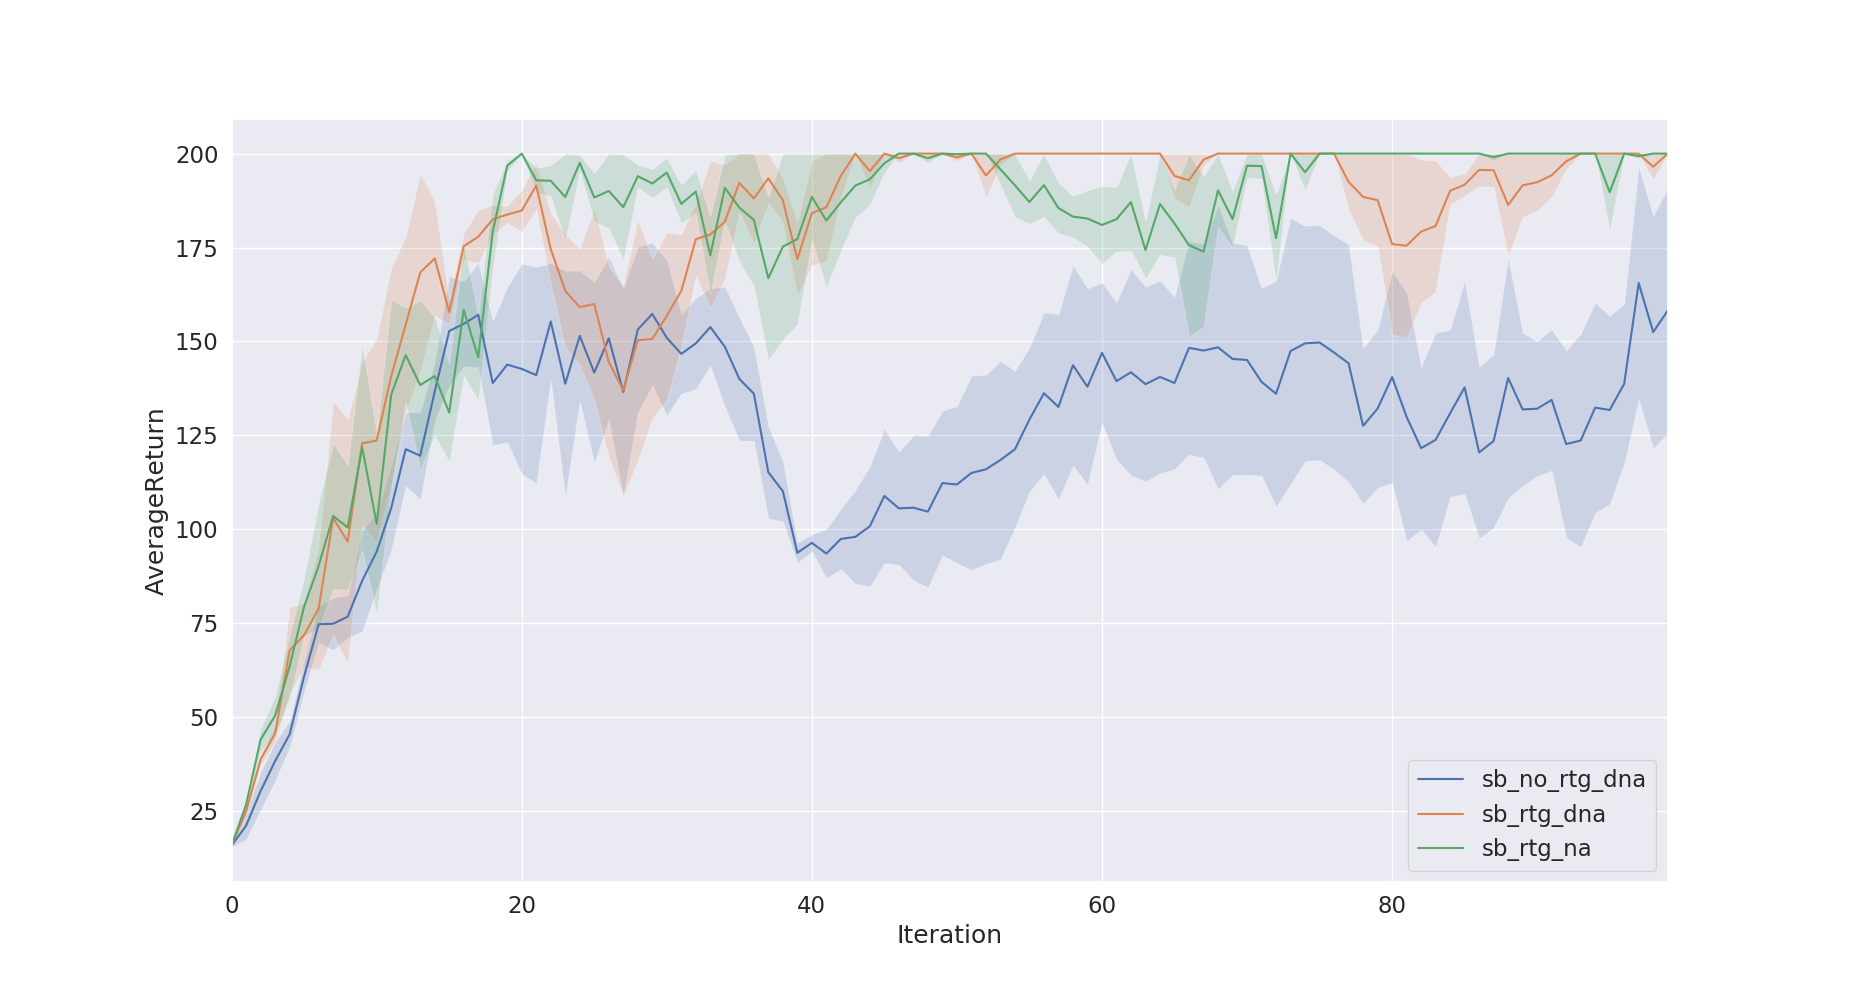
\includegraphics[scale=0.29]{smallBatchCartpole}
    \end{center}

    \subsubsection{Large Batch Performance (CartPole-v0)}
    \begin{center}
        \noindent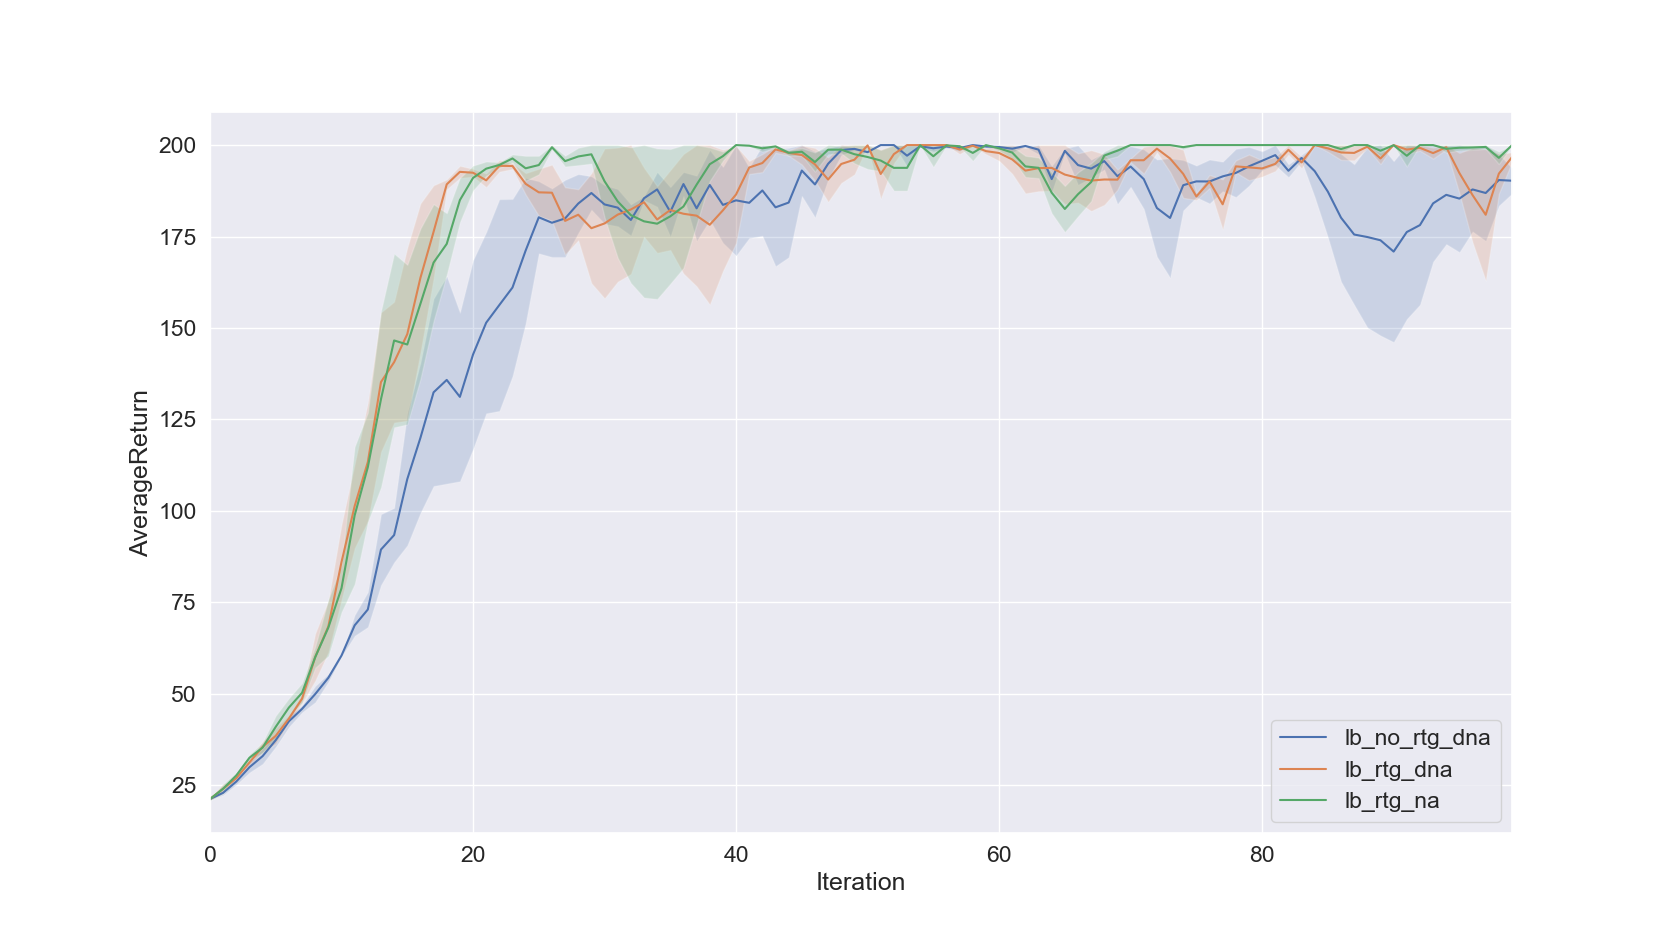
\includegraphics[scale=0.29]{largeBatchCartpole}
    \end{center}

    \subsubsection{Discussion}
    Using reward to go inmproved performance and reduced variance for both 
    small and large batch experiments. Advantage-centering does improve performance.
    Using a larger batch size reduces varaince and speeds up learning for the 
    first few iterations. Both batch sizes were able to converge to near optimal 
    performance, with the exception of the experiment with no variance reduction 
    techniques. In this case, the larger batch size improved performance and reduced 
    variance significantly.

    \subsection{Hyperparameter Tuning (InvertedPendulum-v2)}
    Using a batch size of 400 and learning rate of 0.02, resulted in reaching 
    optimal performance, while minimizing batch size and maximizing learning rate.
    These hyperparameter values were found by grid search over 
    batch sizes $[300, 400, 500]$ and learning rates $[0.03, 0.02, 0.01]$.

    \begin{center}
        \noindent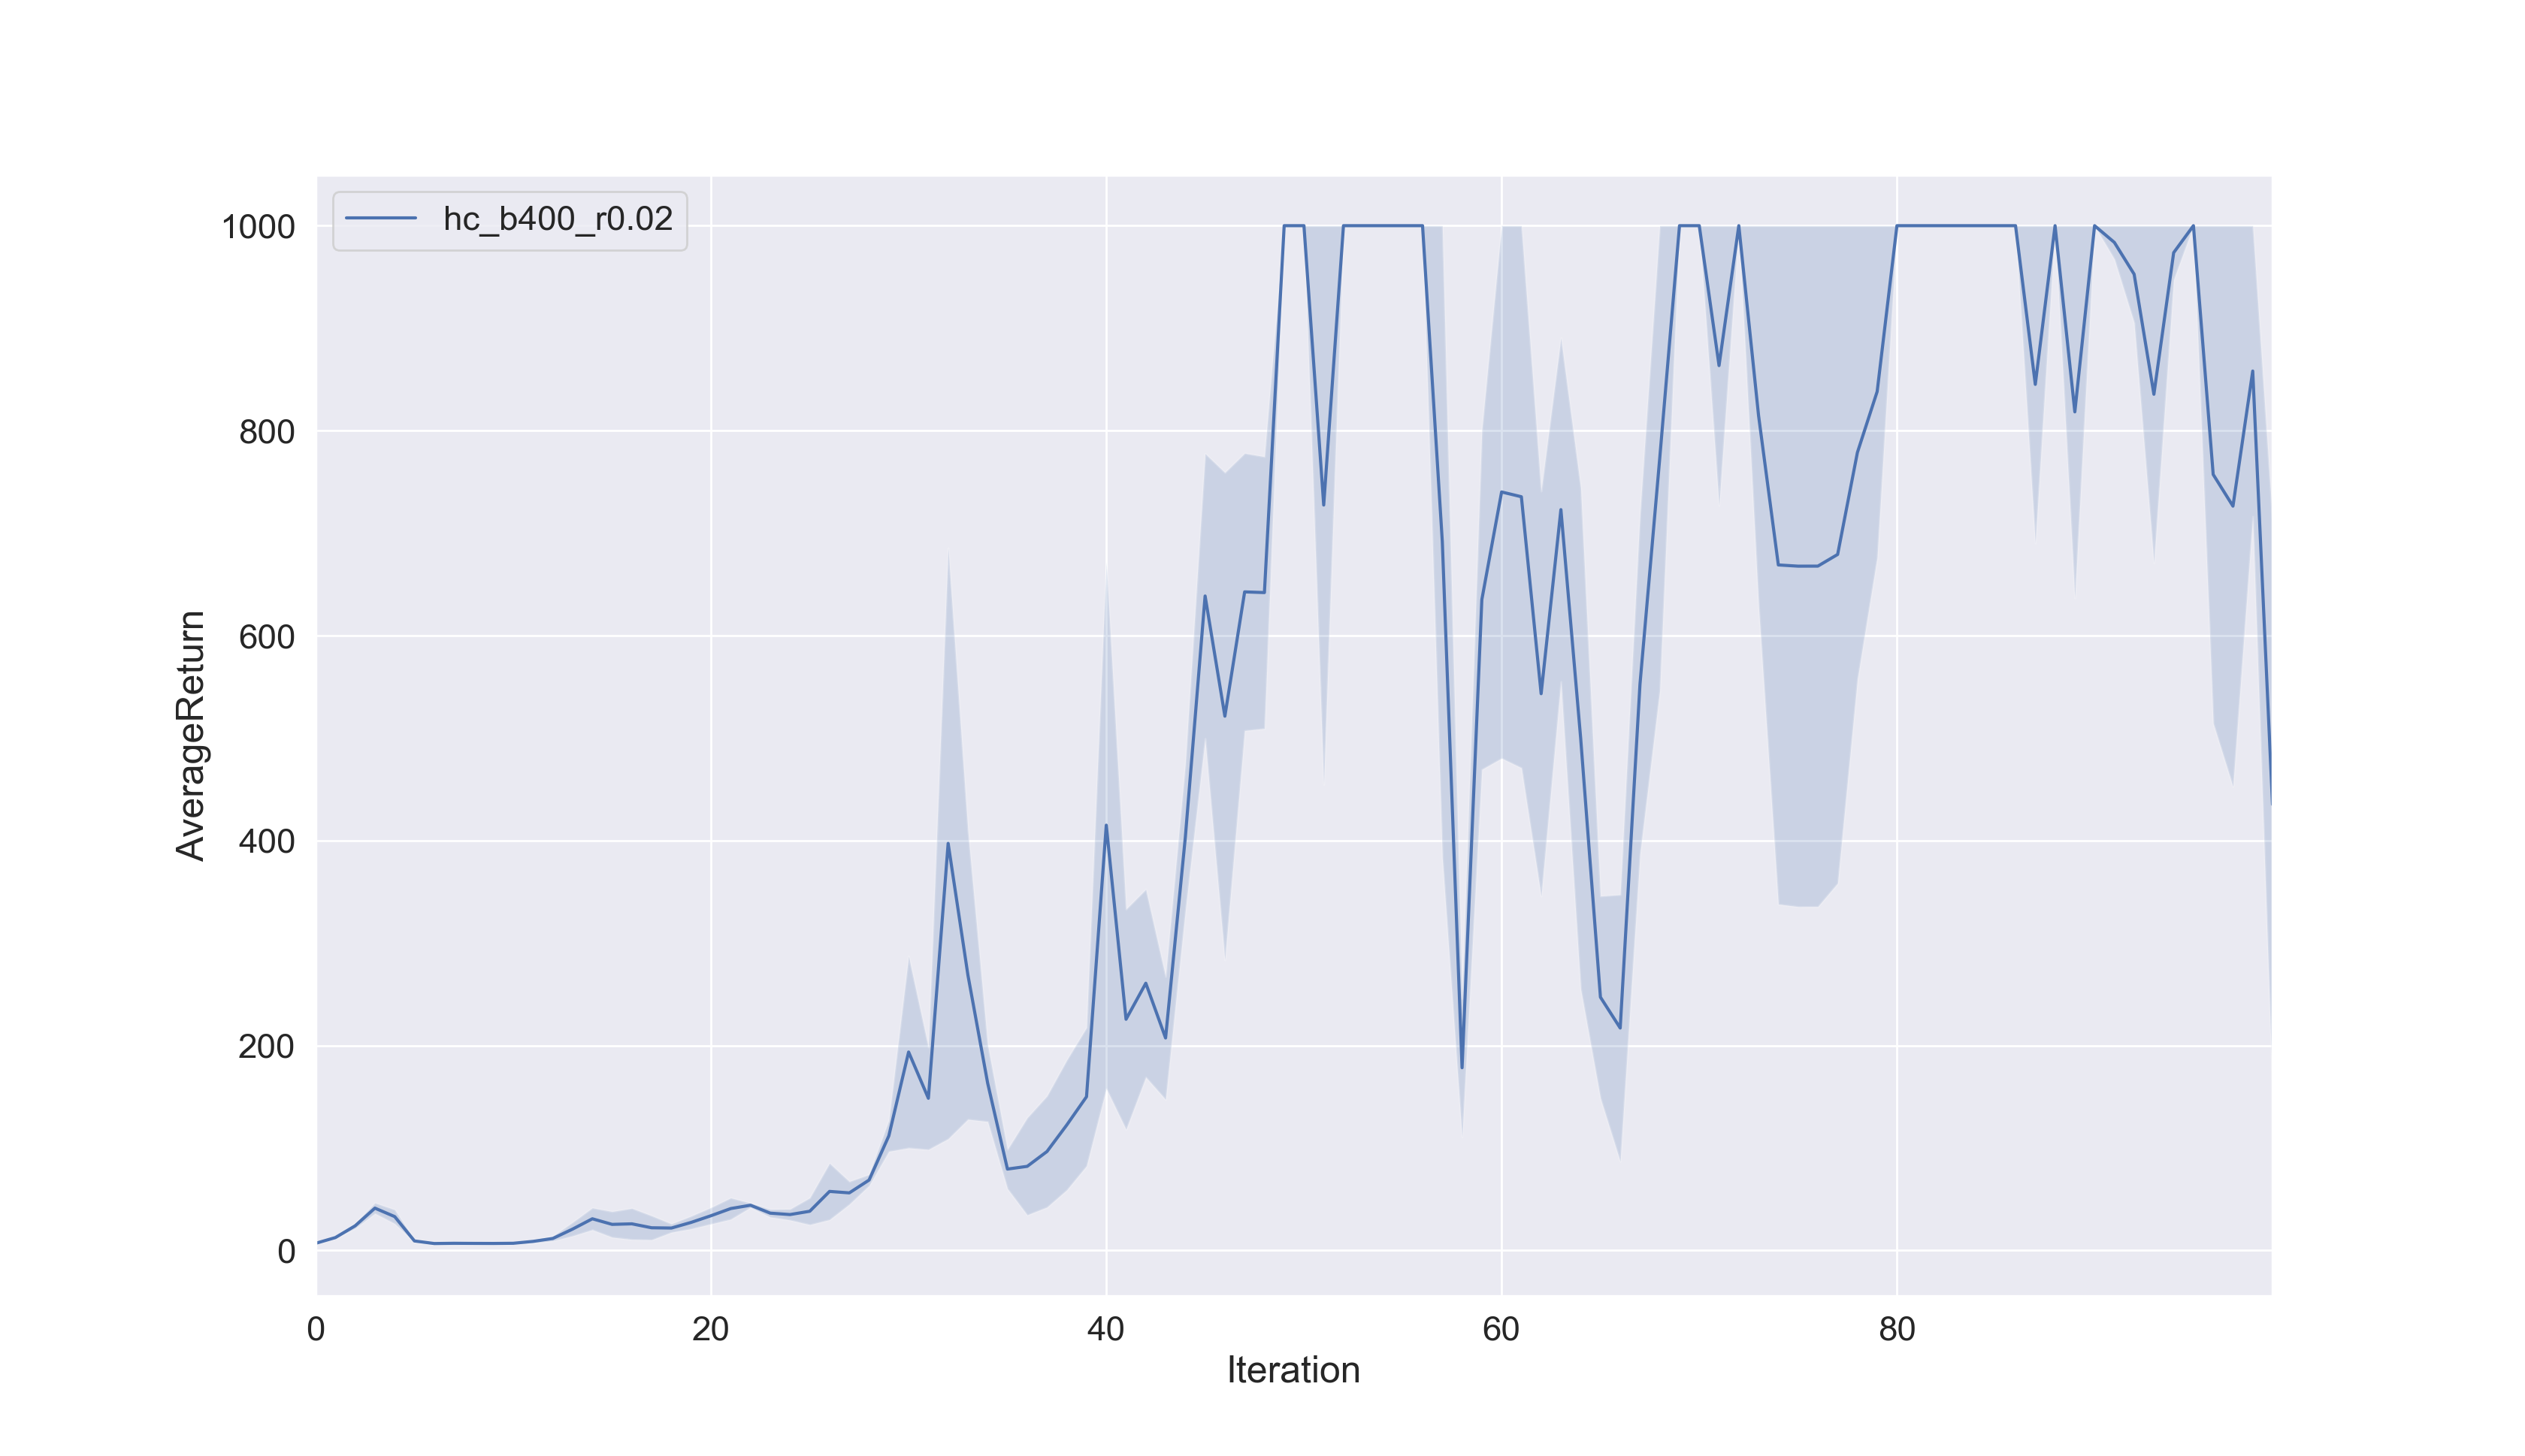
\includegraphics[scale=0.3]{hyperParamsInvertedPendulum}
    \end{center}

    \subsection{Policy Gradient with Baselines}

    \subsubsection{Performance (LunarLander-v2)}
    As expected, using policy gradients with a neural network baseline was 
    able to achieve desired performance. During each policy gradient outer loop, 
    the value network was trained for 100 epochs.
    \begin{center}
        \noindent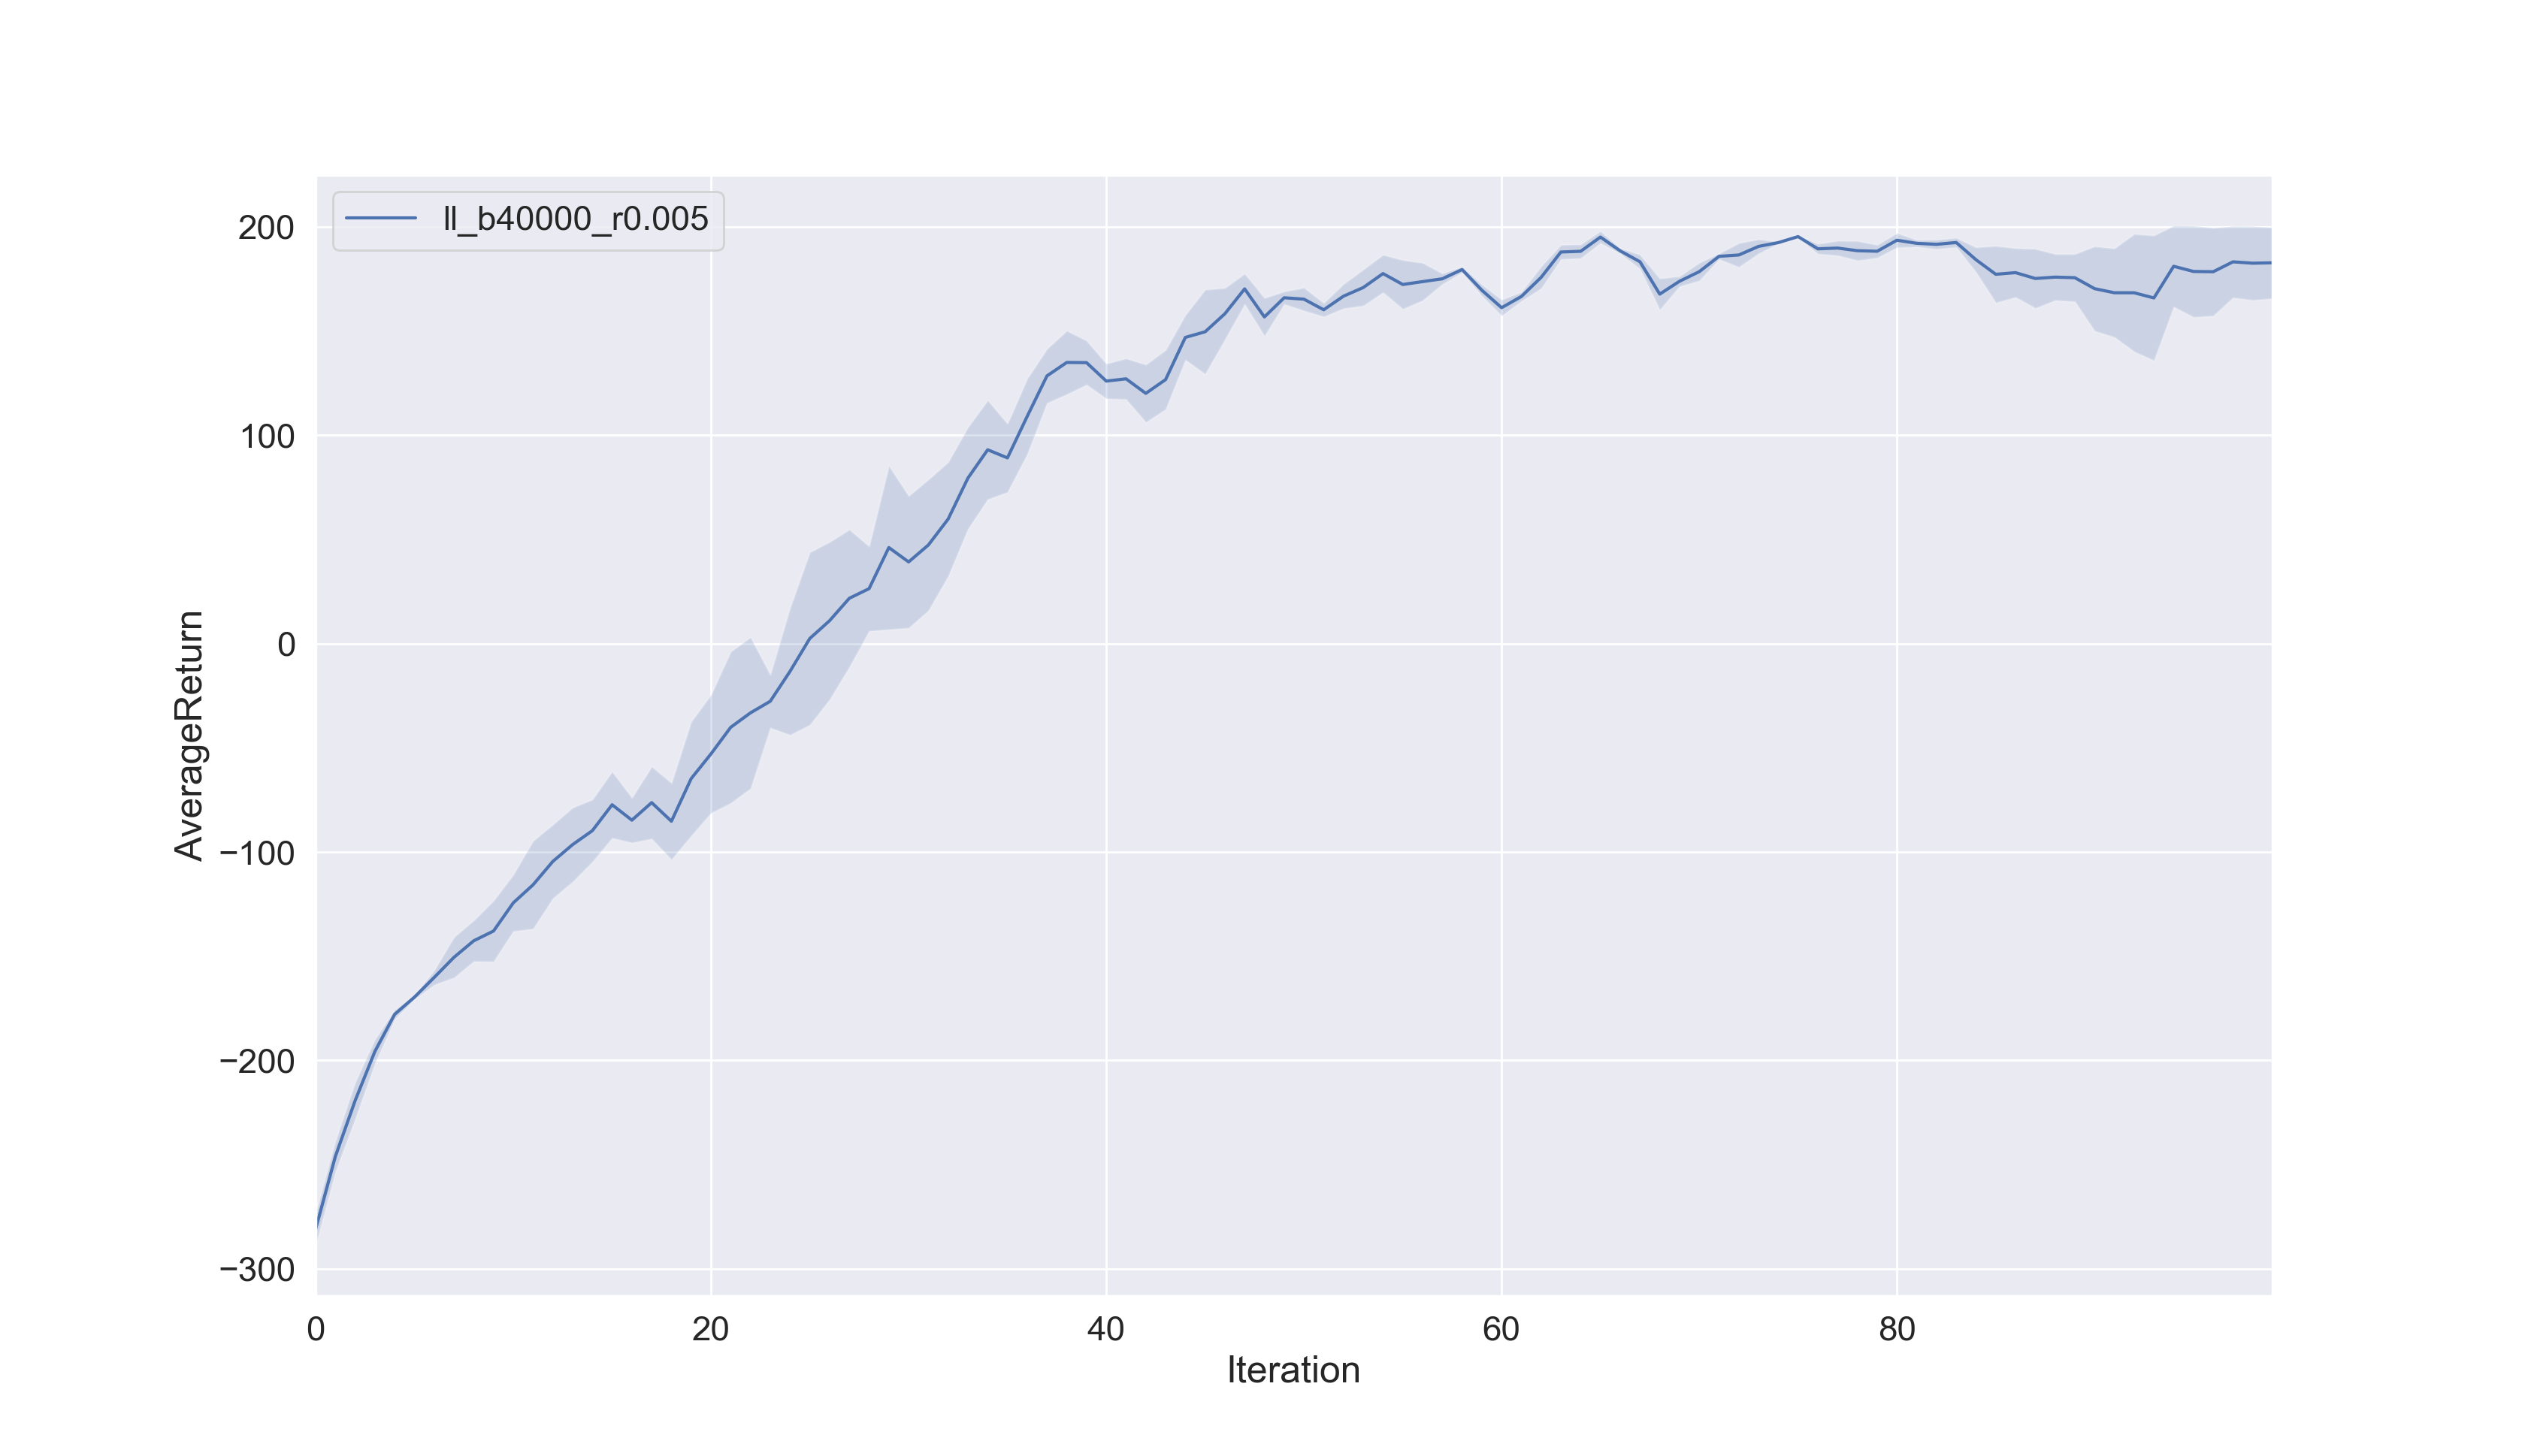
\includegraphics[scale=0.3]{lunarLander}
    \end{center}

    \subsubsection{Hyperparameter Tuning (HalfCheetah-v2)}
    In this experiment, using a higher learning rate results in better performance.
    Increasing batch size also generally improved performance or at least 
    maintained performance. Based on this experiment
    we run the remaining experiments with batch size 50000 and learning rate 0.02.

    \begin{center}
        \noindent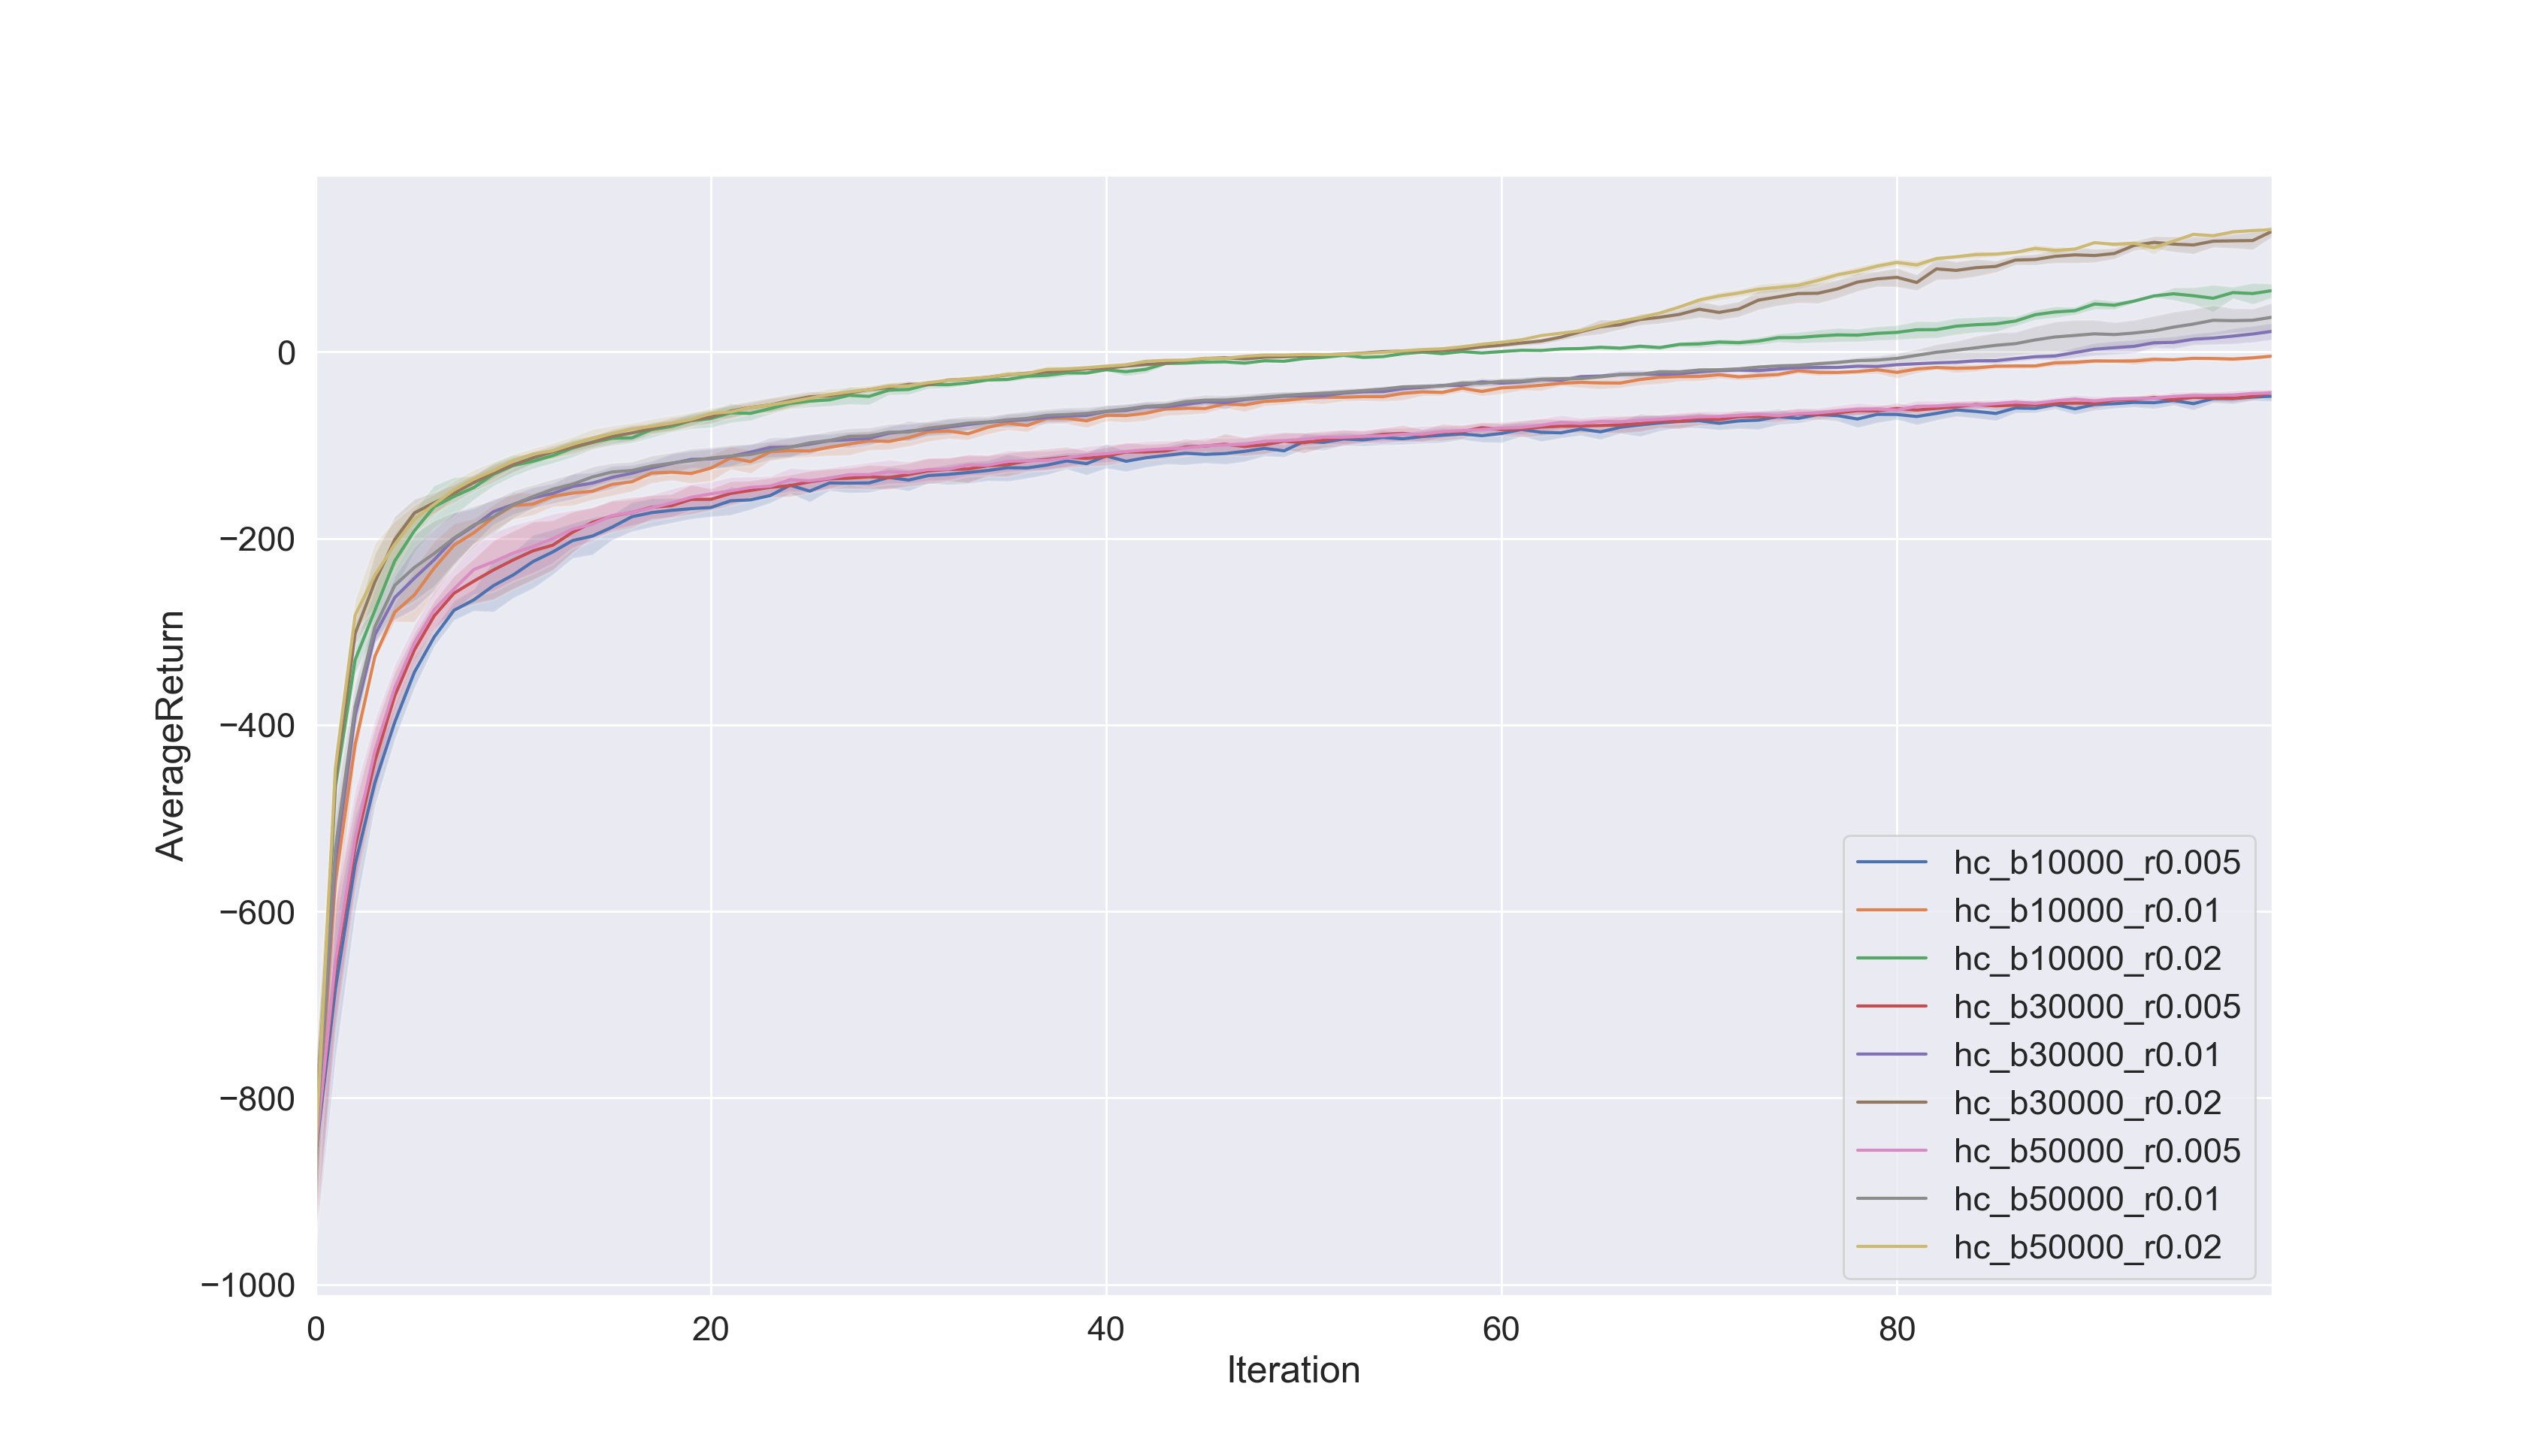
\includegraphics[scale=0.3]{hyperParamsCheetah}
    \end{center}

    \subsubsection{ Performance (HalfCheetah-v2)}
    As shown before using reward to go achieves better performance and lower variance. Using a baseline with 
    reward to go also achieves better performance and significantlt reduces varaince. Using a baseline alone 
    without reward to go performs poorly.
    \begin{center}
        \noindent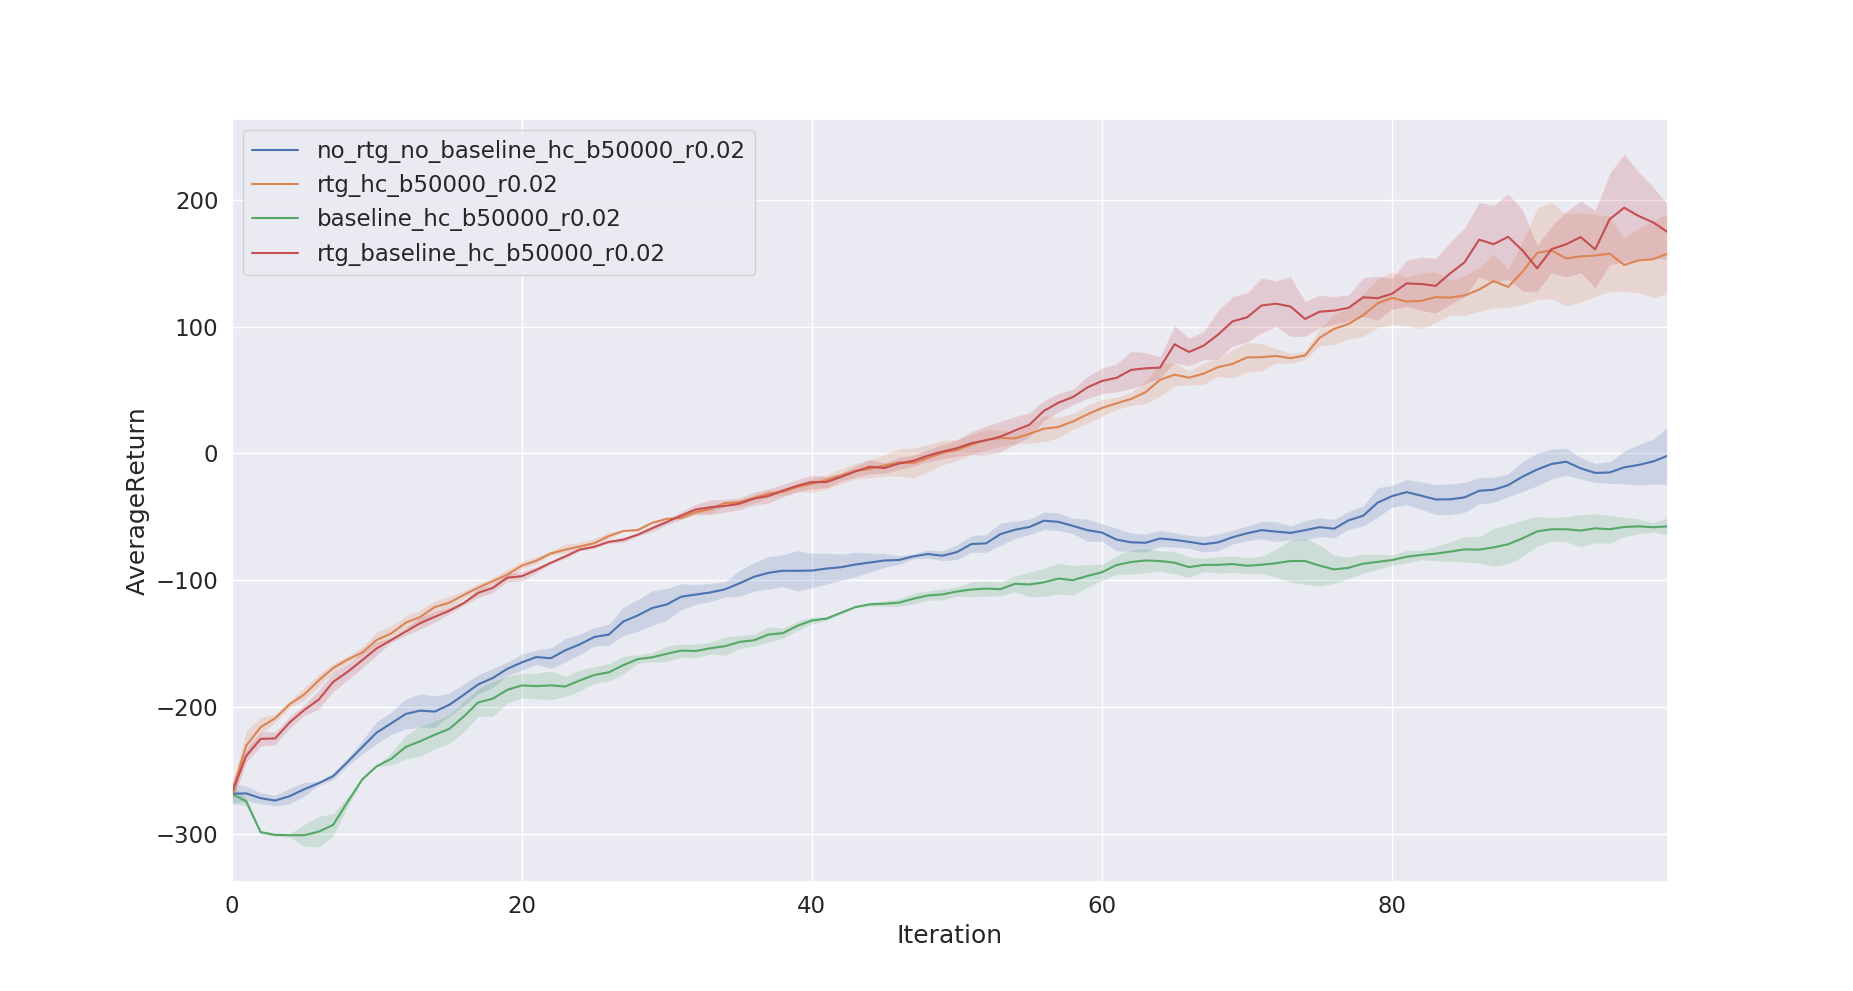
\includegraphics[scale=0.3]{cheetah}
    \end{center}

    \section{Scripts Used}

    To reproduce these results run the following commands from the hw2 directory.

    \begin{verbatim}
        ./p4.sh
        ./p5.sh
        ./p7.sh
        ./p8HyperParamSearch.sh
        ./p8.sh
    \end{verbatim}
\end{document}